\textit{TicTacker} hace uso de diferentes clases que se comunican entre sí y que utilizan los elementos XML de Android para gestionar la vista correspondiente. Adicionalmente, se hace uso de una base de datos MySQL desde un servidor con PHP para gestionar los usuarios, los fichajes, los perfiles, los tokens de FCM y las configuraciones personalizadas.

\subsection{Clases}
La aplicación cuenta con diferentes clases Java diferenciadas que dan respuesta a una o varias de las funcionalidades de la aplicación. A continuación se describen las siguientes clases utilizadas, pudiendo ver las relaciones entre las mismas por medio de diagrama de clases de la Figura \ref{fig:diagrama}.

\subsubsection{Activities}
\begin{itemize}
  \item \textbf{MainActivity}: actividad principal que se encarga de gestionar la navegación y la interfaz de usuario principal de la aplicación.
  \item \textbf{LoginActivity}: gestiona la autentificación de usuarios existentes, validando credenciales y guardando la sesión.
  \item \textbf{SignupActivity}: gestiona el registro de nuevos usuarios, incluyendo validación de los datos, que no se repitan nombres de usuario y creación de cuentas junto con un perfil básico a partir de los datos introducidos.
  \item \textbf{SettingsActivity}: ofrece opciones de personalización de la aplicación, como cambiar el idioma, la jornada laboral, el logotipo o los recordatorios de fichaje.
  \item \textbf{NoInternetActivity}: se lanza en el momento en el que se detecta que no se cuenta con conexión a Internet, bloqueando el uso de la app.
\end{itemize}

\subsubsection{Fragments}
\begin{itemize}
  \item \textbf{ClockInFragment}: fragment que permite a los usuarios registrar sus fichajes, mostrando el estado actual y el tiempo trabajado.
  \item \textbf{FichajeDetailsFragment}: permite a los usuarios ver los detalles de un fichaje concreto seleccionado del historial, dejando ver la ubicación en un mapa de OpenStreetMap en caso de estar disponible.
  \item \textbf{HistoryFragment}: fragment que muestra el historial de fichajes del usuario, permitiendo exportar e importar datos por medio de ficheros CSV.
  \item \textbf{SettingsFragment}: fragment que permite a los usuarios ajustar sus preferencias, como las horas de trabajo semanales y los días laborables.
  \item \textbf{EditFichajeDialog}: dialog fragment utilizado a la hora de editar la hora de entrada y/o salida de un fichaje existente en la aplicación.
\end{itemize}

\subsubsection{Adaptadores}
\begin{itemize}
  \item \textbf{FichajeAdapter}: utilizado para mostrar listas de fichajes a través de un \textit{RecyclerView}.
\end{itemize}

\subsubsection{Clases generales}
\begin{itemize}
  \item \textbf{TicTacker}: clase principal de la aplicación que se encarga de aplicar las preferencias de usuario al iniciar, así como de instanciar OSMdroid para poder utilizar los mapas de OpenStreetMap.
  \item \textbf{Fichaje}: entidad que representa un fichaje con los atributos correspondiente, usado para instanciar objetos fácilmente con su fecha, hora de entrada, hora de salida, latitud, longitud y nombre de usuario para almacenar en la base de datos.
  \item \textbf{WorkTimeCalculator}: clase que proporciona métodos para calcular el tiempo trabajado y el tiempo restante.
  \item \textbf{ApiClient}: clase utilizada para realizar las consultas POST y GET a la API del servidor, permitiendo realizar modificaciones sobre la base de datos.
  \item \textbf{NetworkConnectivityChecker}: clase utilizada para comprobar si se tiene conexión a Internet al ser requerida para funcionar. En caso de no tener conexión, se lanza \textit{NoInternetActivity}.
  \item \textbf{UserProfile}: clase utilizada para gestionar los perfiles de usuario, almacenando valores como el nombre, el email o la foto de perfil.
\end{itemize}

\subsubsection{Helpers}
\begin{itemize}
  \item \textbf{DatabaseHelper}: gestiona la base de datos MySQL realizando llamadas al \textit{DatabaseWorker} que, a su vez, utiliza \textit{ApiClient} para llamar a la API y hacer cambios en el servidor.
  \item \textbf{NotificationHelper}: clase que gestiona la creación y envío de notificaciones.
\end{itemize}

\subsubsection{Receivers}
\begin{itemize}
  \item \textbf{BootReceiver}: clase auxiliar utilizada para reconfigurar las alarmas de los recordatorios de fichajes en caso de que el dispositivo se reinicie.
  \item \textbf{ClockInReminderReceiver}: clase que interpreta y gestiona las alarmas enviadas por la clase \textit{ClockInReminderService} y que se encarga de generar las notificaciones de recordatorios de fichajes.
\end{itemize}

\subsubsection{Services}
\begin{itemize}
  \item \textbf{ClockInReminderService}: clase utilizada para enviar alarmas para recordar al usuario que inicie un fichaje si se supera una hora determinada y no se ha fichado.
  \item \textbf{ForegroundTimeService}: servicio empleado para gestionar la actividad de fichaje en primer plano (\textit{Foreground}), lanzando una notificación silenciosa persistente para informar del estado del fichaje.
  \item \textbf{MyFirebaseMessagingService}: servicio utilizado para registrar los tokens FCM de Firebase y recibir notificaciones enviadas a distancia.
\end{itemize}

\subsubsection{Eventos}
\begin{itemize}
  \item \textbf{FichajeEvents}: clase que gestiona los eventos relacionados con los fichajes, permitiendo notificar cambios a los listeners registrados.
\end{itemize}

\subsubsection{Widgets}
\begin{itemize}
  \item \textbf{TicTackerWidget}: clase utilizada para gestionar todos los aspectos relacionados con el widget de la aplicación.
\end{itemize}

\subsubsection{Workers}
\begin{itemize}
  \item \textbf{DatabaseWorker}: worker que envía y recibe las consultas en formato JSON realizadas a la API para realizar cambios sobre la base de datos.
  \item \textbf{WorkTimeCheckWorker}: worker que comprueba periódicamente el tiempo trabajado y envía notificaciones al usuario si alcanza su jornada laboral.
\end{itemize}

\begin{figure}[H]
    \centering
    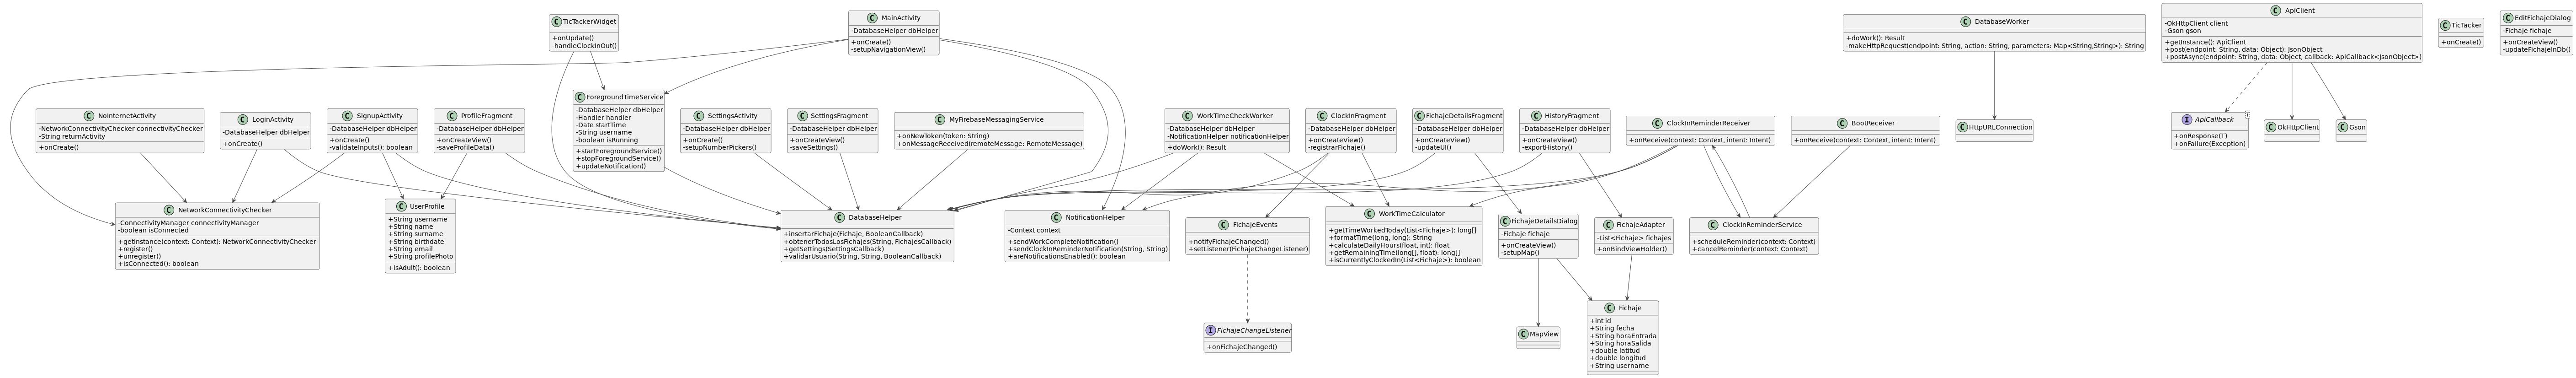
\includegraphics[width=1\linewidth]{root/diagrama.png}
    \caption{Diagrama de clases del proyecto}
    \label{fig:diagrama}
\end{figure}

\subsection{Base de datos}

Además de las \textit{SharedPreferences}, para gestionar la persistencia de la aplicación se hace uso de una base de datos de tipo MySQL controlada desde un servidor PHP, que tal y como se muestra en el diagrama de la Figura \ref{fig:bd}, contiene las siguientes tablas:

\begin{itemize}
  \item \textbf{Tabla \texttt{fichajes}}: almacena la información sobre los fichajes de los usuarios.
  \begin{itemize}
    \item \textbf{Atributos principales}: \texttt{id}, \texttt{fecha}, \texttt{hora\_entrada}, \texttt{hora\_salida}, \texttt{latitud}, \texttt{longitud}, \texttt{username}.
    \item \textbf{Índices}: \texttt{id} es un campo único y clave primaria.
  \end{itemize}
  
  \item \textbf{Tabla \texttt{users}}: almacena los usuarios registrados en la aplicación.
  \begin{itemize}
    \item \textbf{Atributos principales}: \texttt{id}, \texttt{username}, \texttt{password}.
    \item \textbf{Índices}: \texttt{username} es un campo único indexado para prevenir duplicados.
  \end{itemize}
  
  \item \textbf{Tabla \texttt{settings}}: almacena las configuraciones de horas de trabajo y recordatorios.
  \begin{itemize}
    \item \textbf{Atributos principales}: \texttt{id}, \texttt{weekly\_hours}, \texttt{working\_days}, \texttt{reminder\_enabled}, \texttt{reminder\_hour}, \texttt{reminder\_minute}.
    \item \textbf{Índices}: \texttt{id} es un campo único y clave primaria.
  \end{itemize}
  
  \item \textbf{Tabla \texttt{fcm\_tokens}}: almacena los tokens de notificaciones push para cada usuario.
  \begin{itemize}
    \item \textbf{Atributos principales}: \texttt{id}, \texttt{username}, \texttt{token}, \texttt{created\_at}, \texttt{updated\_at}.
    \item \textbf{Índices}: \texttt{id} es un campo único y clave primaria.
  \end{itemize}

  \item \textbf{Tabla \texttt{user\_profiles}}: almacena información adicional del perfil del usuario.
  \begin{itemize}
    \item \textbf{Atributos principales}: \texttt{id}, \texttt{username}, \texttt{name}, \texttt{surname}, \texttt{birthdate}, \texttt{email}, \texttt{profile\_photo}.
    \item \textbf{Índices}: \texttt{id} es un campo único y clave primaria.
  \end{itemize}
\end{itemize}

\begin{figure}[H]
    \centering
    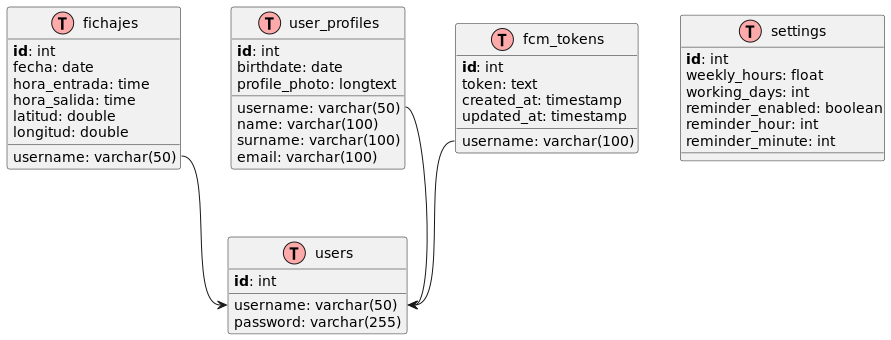
\includegraphics[width=1\linewidth]{root/bd.png}
    \caption{Diagrama de la base de datos usada del proyecto}
    \label{fig:bd}
\end{figure}

\subsection{Ficheros PHP usados en el servidor}

Para ejecutar consultas sobre la base de datos MySQL mencionada anteriormente, así como realizar los correspondientes envíos de la mensajería FCM, se han cargado a través de SFTP los siguientes ficheros en la dirección de Internet \url{http://ec2-51-44-167-78.eu-west-3.compute.amazonaws.com/ffernandez032/WEB/}, disponibles para su consulta en el \href{https://github.com/ffernandezco/TicTacker/tree/main/server}{directorio \texttt{server} del repositorio de GitHub}:

\begin{itemize}
  \item \textbf{db\_connect.php}: recoge las credenciales de conexión a la base de datos. Por motivos de seguridad, se han ocultado algunos campos en el repositorio de GitHub. Modificando los ficheros y las direcciones de la conexión es posible usar otro servidor si así se desea.
  \item \textbf{auth\_user.php}: verifica que un usuario y contraseña coinciden con el \textit{hash} almacenado en la base de datos para permitir su autenticación.
  \item \textbf{fcm\_tokens.php}: se encarga de almacenar los tokens FCM de Firebase y de actualizar si es necesario el usuario al que está asociado cada uno.
  \item \textbf{fichajes.php}: gestiona todas las operaciones relacionadas con los fichajes, incluyendo añadirlos, modificarlos o eliminarlos.
  \item \textbf{firebase\_service\_account.json}: fichero extraído del gestor de cuentas de servicio IAM de Google que contiene los datos necesarios para enviar mensajes usando la mensajería Cloud Messagging de Firebase. Por motivos de seguridad, no se ha incluido en el repositorio de GitHub.
  \item \textbf{jwt\_utils.php}: adaptación compilada del \href{https://github.com/firebase/php-jwt}{repositorio \texttt{firebase/php-jwt}} para gestionar la autenticación de Firebase desde PHP.
  \item \textbf{notificar.php}: habilita una interfaz HTML que permite enviar una notificación a todos los usuarios con un token FCM almacenado en la base de datos. Está disponible de forma pública en la dirección \url{http://ec2-51-44-167-78.eu-west-3.compute.amazonaws.com/ffernandez032/WEB/notificar.php}.
  \item \textbf{profile.php}: gestiona todas las operaciones relacionadas con los perfiles de usuario, como modificar o añadir el nombre, los apellidos, la foto de perfil o el correo electrónico.
  \item \textbf{send\_notification\_v1.php}: permite enviar notificaciones a los usuarios a través del token usando Firebase Cloud Messagging (FCM).
  \item \textbf{settings.php}: gestiona todas las operaciones relacionadas con las configuraciones, como la configuración de la jornada o el envío de notificaciones.
  \item \textbf{users.php}: gestiona todas las operaciones relacionadas con los usuarios, como añadir un usuario o modificar la contraseña asociada.
\end{itemize}